\documentclass[10pt]{article}
\usepackage[T1]{fontenc}

% Document Details
\newcommand{\CLASS}{AMATH 586}
\newcommand{\assigmentnum}{Assignment 2}

\usepackage[margin = 1.15in, top = 1.25in, bottom = 1.in]{geometry}

\usepackage{titling}
\setlength{\droptitle}{-6em}   % This is your set screw
\date{}
\renewcommand{\maketitle}{
	\clearpage
	\begingroup  
	\centering
	\LARGE \sffamily\textbf{\CLASS} \Large \assigmentnum\\[.8em]
	\large Tyler Chen\\[1em]
	\endgroup
	\thispagestyle{empty}
}
 % Title Styling
\usepackage{tocloft}
\renewcommand{\cfttoctitlefont}{\Large\sffamily\bfseries}
\renewcommand{\cftsecfont}{\normalfont\sffamily\bfseries}
\renewcommand{\cftsubsecfont}{\normalfont\sffamily}
\renewcommand{\cftsubsubsecfont}{\normalfont\sffamily}

\makeatletter
\let\oldl@section\l@section
\def\l@section#1#2{\oldl@section{#1}{\sffamily\bfseries#2}}

\let\oldl@subsection\l@subsection
\def\l@subsection#1#2{\oldl@subsection{#1}{\sffamily#2}}

\let\oldl@subsubsection\l@subsubsection
\def\l@subsubsection#1#2{\oldl@subsubsection{#1}{\sffamily#2}}
 % General Styling


\usepackage{enumitem}

% Figures
\usepackage{subcaption}

% TikZ and Graphics
\usepackage{tikz, pgfplots}
\pgfplotsset{compat=1.12}
\usetikzlibrary{patterns,arrows}
\usepgfplotslibrary{fillbetween}

\usepackage{pdfpages}
\usepackage{adjustbox}

\usepackage{lscape}
\usepackage{titling}
\usepackage[]{hyperref}


% Header Styling
\usepackage{fancyhdr}
\pagestyle{fancy}
\lhead{\sffamily \CLASS}
\rhead{\sffamily Chen \textbf{\thepage}}
\cfoot{}

% Paragraph Styling
\setlength{\columnsep}{1cm}
\setlength{\parindent}{0pt}
\setlength{\parskip}{5pt}
\renewcommand{\baselinestretch}{1}

% TOC Styling
\usepackage{tocloft}
\iffalse
\renewcommand{\cftsecleader}{\cftdotfill{\cftdotsep}}

\renewcommand\cftchapafterpnum{\vskip6pt}
\renewcommand\cftsecafterpnum{\vskip10pt}
\renewcommand\cftsubsecafterpnum{\vskip6pt}

% Adjust sectional unit title fonts in ToC
\renewcommand{\cftchapfont}{\sffamily}
\renewcommand{\cftsecfont}{\bfseries\sffamily}
\renewcommand{\cftsecnumwidth}{2em}
\renewcommand{\cftsubsecfont}{\sffamily}
\renewcommand{\cfttoctitlefont}{\hfill\bfseries\sffamily\MakeUppercase}
\renewcommand{\cftaftertoctitle}{\hfill}

\renewcommand{\cftchappagefont}{\sffamily}
\renewcommand{\cftsecpagefont}{\bfseries\sffamily}
\renewcommand{\cftsubsecpagefont}{\sffamily}
\fi
 % General Styling
% Code Display Setup
\usepackage{listings,lstautogobble}
\usepackage{lipsum}
\usepackage{courier}
\usepackage{catchfilebetweentags}

\lstset{
	basicstyle=\small\ttfamily,
	breaklines=true, 
	frame = single,
	rangeprefix=,
	rangesuffix=,
	includerangemarker=false,
	autogobble = true
}


\usepackage{algorithmicx}
\usepackage{algpseudocode}

\newcommand{\To}{\textbf{to}~}
\newcommand{\DownTo}{\textbf{downto}~}
\renewcommand{\algorithmicdo}{\hspace{-.2em}\textbf{:}}
 % Code Display Setup
% AMS MATH Styling
\usepackage{amsmath, amssymb}
\newcommand{\qed}{\hfill\(\square\)}

%\newtheorem*{lemma}{Lemma} 
%\newtheorem*{theorem}{Theorem}
%\newtheorem*{definition}{Definition}
%\newtheorem*{prop}{Proposition}
%\renewenvironment{proof}{{\bfseries Proof.}}{}


% mathcal
\newcommand{\cA}{\ensuremath{\mathcal{A}}}
\newcommand{\cB}{\ensuremath{\mathcal{B}}}
\newcommand{\cC}{\ensuremath{\mathcal{C}}}
\newcommand{\cD}{\ensuremath{\mathcal{D}}}
\newcommand{\cE}{\ensuremath{\mathcal{E}}}
\newcommand{\cF}{\ensuremath{\mathcal{F}}}
\newcommand{\cG}{\ensuremath{\mathcal{G}}}
\newcommand{\cH}{\ensuremath{\mathcal{H}}}
\newcommand{\cI}{\ensuremath{\mathcal{I}}}
\newcommand{\cJ}{\ensuremath{\mathcal{J}}}
\newcommand{\cK}{\ensuremath{\mathcal{K}}}
\newcommand{\cL}{\ensuremath{\mathcal{L}}}
\newcommand{\cM}{\ensuremath{\mathcal{M}}}
\newcommand{\cN}{\ensuremath{\mathcal{N}}}
\newcommand{\cO}{\ensuremath{\mathcal{O}}}
\newcommand{\cP}{\ensuremath{\mathcal{P}}}
\newcommand{\cQ}{\ensuremath{\mathcal{Q}}}
\newcommand{\cR}{\ensuremath{\mathcal{R}}}
\newcommand{\cS}{\ensuremath{\mathcal{S}}}
\newcommand{\cT}{\ensuremath{\mathcal{T}}}
\newcommand{\cU}{\ensuremath{\mathcal{U}}}
\newcommand{\cV}{\ensuremath{\mathcal{V}}}
\newcommand{\cW}{\ensuremath{\mathcal{W}}}
\newcommand{\cX}{\ensuremath{\mathcal{X}}}
\newcommand{\cY}{\ensuremath{\mathcal{Y}}}
\newcommand{\cZ}{\ensuremath{\mathcal{Z}}}

% mathbb
\usepackage{bbm}
\newcommand{\bOne}{\ensuremath{\mathbbm{1}}}

\newcommand{\bA}{\ensuremath{\mathbb{A}}}
\newcommand{\bB}{\ensuremath{\mathbb{B}}}
\newcommand{\bC}{\ensuremath{\mathbb{C}}}
\newcommand{\bD}{\ensuremath{\mathbb{D}}}
\newcommand{\bE}{\ensuremath{\mathbb{E}}}
\newcommand{\bF}{\ensuremath{\mathbb{F}}}
\newcommand{\bG}{\ensuremath{\mathbb{G}}}
\newcommand{\bH}{\ensuremath{\mathbb{H}}}
\newcommand{\bI}{\ensuremath{\mathbb{I}}}
\newcommand{\bJ}{\ensuremath{\mathbb{J}}}
\newcommand{\bK}{\ensuremath{\mathbb{K}}}
\newcommand{\bL}{\ensuremath{\mathbb{L}}}
\newcommand{\bM}{\ensuremath{\mathbb{M}}}
\newcommand{\bN}{\ensuremath{\mathbb{N}}}
\newcommand{\bO}{\ensuremath{\mathbb{O}}}
\newcommand{\bP}{\ensuremath{\mathbb{P}}}
\newcommand{\bQ}{\ensuremath{\mathbb{Q}}}
\newcommand{\bR}{\ensuremath{\mathbb{R}}}
\newcommand{\bS}{\ensuremath{\mathbb{S}}}
\newcommand{\bT}{\ensuremath{\mathbb{T}}}
\newcommand{\bU}{\ensuremath{\mathbb{U}}}
\newcommand{\bV}{\ensuremath{\mathbb{V}}}
\newcommand{\bW}{\ensuremath{\mathbb{W}}}
\newcommand{\bX}{\ensuremath{\mathbb{X}}}
\newcommand{\bY}{\ensuremath{\mathbb{Y}}}
\newcommand{\bZ}{\ensuremath{\mathbb{Z}}}

% alternative mathbb
\newcommand{\NN}{\ensuremath{\mathbb{N}}}
\newcommand{\RR}{\ensuremath{\mathbb{R}}}
\newcommand{\CC}{\ensuremath{\mathbb{C}}}
\newcommand{\ZZ}{\ensuremath{\mathbb{Z}}}
\newcommand{\EE}{\ensuremath{\mathbb{E}}}
\newcommand{\PP}{\ensuremath{\mathbb{P}}}
\newcommand{\VV}{\ensuremath{\mathbb{V}}}
\newcommand{\cov}{\ensuremath{\text{Co}\VV}}
% Math Commands

\newcommand{\st}{~\big|~}
\newcommand{\stt}{\text{ st. }}
\newcommand{\ift}{\text{ if }}
\newcommand{\thent}{\text{ then }}
\newcommand{\owt}{\text{ otherwise }}

\newcommand{\norm}[1]{\left\lVert#1\right\rVert}
\newcommand{\snorm}[1]{\lVert#1\rVert}
\newcommand{\ip}[1]{\ensuremath{\left\langle #1 \right\rangle}}
\newcommand{\pp}[3][]{\frac{\partial^{#1}#2}{\partial #3^{#1}}}
\newcommand{\dd}[3][]{\frac{\d^{#1}#2}{\d #3^{#1}}}
\renewcommand{\d}{\ensuremath{\mathrm{d}}}

\newcommand{\indep}{\rotatebox[origin=c]{90}{$\models$}}




 % Math shortcuts
% Problem
\usepackage{floatrow}

\newenvironment{problem}[1][]
{\pagebreak
\noindent\rule{\textwidth}{1pt}\vspace{0.25em}
{\sffamily \textbf{#1}}
\par
}
{\par\vspace{-0.5em}\noindent\rule{\textwidth}{1pt}}

\newenvironment{solution}[1][]
{{\sffamily \textbf{#1}}
\par
}
{}

 % Problem Environment

\newcommand{\note}[1]{\textcolor{red}{\textbf{Note:} #1}}

\hypersetup{
   colorlinks=true,       % false: boxed links; true: colored links
   linkcolor=violet,          % color of internal links (change box color with linkbordercolor)
   citecolor=green,        % color of links to bibliography
   filecolor=magenta,      % color of file links
   urlcolor=cyan           % color of external links
}


\begin{document}
\maketitle



\begin{problem}[Preliminaries]
Recall the general expression for a \( r \)-step LMM,
\begin{align*}
    \sum_{j=0}^{r} \alpha_j U^{n+j} = k \sum_{j=0}^{r} \beta_j f(U^{n+j},t_{n+j})
\end{align*}
The local truncation error is,
\begin{align*}
    \tau_{n+2} = \dfrac{1}{k}\left( \sum_{j=0}^{r} \alpha_j \right)u(t_n) + \sum_{q=1}^{\infty}\left(k^{q-1} \left(\sum_{j=0}^{2} \left(\dfrac{1}{q!}j^q\alpha_j -\dfrac{1}{(q-1)!}j^{q-1} \beta_j\right)\right)u^{(q)}(t_n)\right)
\end{align*}
Note that for any integer \( q>0 \),
\begin{align*}
    k^{q-1} \left(\sum_{j=0}^{r} \left(\dfrac{1}{q!}j^q\alpha_j -\dfrac{1}{(q-1)!}j^{q-1} \beta_j\right)\right)u^{(q)}(t_n) = 0
     && \Longleftrightarrow &&
    \sum_{j=0}^{r} j^q \alpha_j = q\sum_{j=0}^{r}j^{q-1} \beta_j
\end{align*}

\end{problem}


\begin{problem}[Problem 1]
Determine the coefficients \(\beta_0\), \(\beta_1\), \(\beta_2\) for the third order, 2-step Adams-Moulton method:
\[
U^{n+2} = U^{n+1} + k [ \beta_0 f( U^n , t_n ) + \beta_1 f( U^{n+1} , t_{n+1} ) +
\beta_2 f( U^{n+2} , t_{n+2} ) ] .
\]
Do this in two different ways:
\begin{enumerate}[label=(\alph*)]
\item Using the expression for the local truncation error in Section 5.9.1.
\item Using the relation
\[
u( t_{n+2} ) = u( t_{n+1} ) + \int_{t_{n+1}}^{t_{n+2}} f( u(s),s )\,ds ,
\]
and replacing \(f\) in the integral by a quadratic polynomial \(p(s)\) that takes the values
\(f( U^n , t_n )\), \(f( U^{n+1} , t_{n+1} )\), and \(f( U^{n+2} , t_{n+2} )\) at the points \(t_n\),
\(t_{n+1}\), and \(t_{n+2}\).
\end{enumerate}
\end{problem}

\begin{solution}[Solution]

\begin{enumerate}[label=(\alph*)]
    \item This is a 2-step LMM with \( \alpha_0 = 0\), \(\alpha_1 = -1\), and \( \alpha_2 = 1 \).

     Clearly \( \sum_{j=0}^{2} \alpha_j = 0 \). We have three unknowns, so we hope to satisfy at least 3 of the equations. The first three equations are,
     \begin{align*}
        \sum_{j=0}^{2} j \alpha_j = \sum_{j=0}^{2} \beta_j, &&
        \sum_{j=0}^{2} j^2 \alpha_j = 2\sum_{j=0}^{2} j\beta_j, &&
        \sum_{j=0}^{2} j^3 \alpha_j = 3\sum_{j=0}^{2} j^2\beta_j
     \end{align*}

     This gives the linear system,
     \begin{align*}
         \left[\begin{array}{ccc}
         1 & 1 &  1 \\
         0 & 2\cdot 1^1 & 2\cdot2^1 \\
         0 & 3\cdot1^2 & 3\cdot2^2
         \end{array}\right]
         \left[\begin{array}{c} \beta_0 \\ \beta_1 \\ \beta_2 \end{array}\right]
         =
         \left[\begin{array}{c}
         1^1\alpha_1 +2^1\alpha_2 \\
         1^2\alpha_1 + 2^2\alpha_2 \\
         1^3\alpha_1 + 2^3\alpha_2
         \end{array}\right]
         =
         \left[\begin{array}{c} 1 \\ 3 \\ 7 \end{array}\right]
     \end{align*}

     This has solution,
     \begin{align*}
         \beta_0 = -1/12, &&
         \beta_1 = 2/3 , &&
         \beta_2 = 5/12
     \end{align*}

     \item
     We approximate \( f(u(s),s) \) with a polynomial \( F(x) \) passing through the points \( f_n := (f(u(t_n),t_n) \), \( f_{n+1}:=(f(u(t_{n+1}),t_{n+1}) \), and \( f_{n+2}:=(f(u(t_{n+2}),t_{n+2}) \). In particular, this is the Lagrange interpolating polynomial, with equation,
     \begin{align*}
         P(s) = f_n  \dfrac{(s-t_{n+1})(s-t_{n+2})}{(t_n-t_{n+1})(t_n-t_{n+2})}
         + f_{n+1}  \dfrac{(s-t_{n})(s-t_{n+2})}{(t_{n+1}-t_n)(t_{n+1}-t_{n+2})}
         + f_{n+2}  \dfrac{(s-t_{n})(s-t_{n+1})}{(t_{n+2}-t_{n})(t_{n+2}-t_{n+1})}
     \end{align*}

     With the assumption that \( k = t_{n+2}-t_{n+1} = t_{n+1} - t_n \) we easily compute (using Mathematica),
     \begin{align*}
         \int_{t_{n+1}}^{t_{n+2}} P(s) \d s = \dfrac{k}{12} \left( - f(U^n,t_n) + 8f(U^{n+1},t_{n+1}) + 5f(U^{n+2},t_{n+2})  \right)
     \end{align*}

     Using this approximation of the integral to construct a 2-step LMM gives the coefficients,
     \begin{align*}
         \beta_0 = -1/12, &&
         \beta_1 = 2/3, &&
         \beta_2 = 5/12
     \end{align*}


\end{enumerate}

\end{solution}

\begin{problem}[Problem 2]
What is the order of the local truncation error for each of the following linear multistep methods, and which of these methods are {\em convergent}?  Justify your answers.
\begin{enumerate}[label=(\alph*)]
\item \(U^{n} - U^{n-2} = k[ f( U^n , t_n ) - 3 f( U^{n-1} , t_{n-1} ) + 4 f( U^{n-2} , t_{n-2} ) ]\).
\item \(U^n - 2 U^{n-1} + U^{n-2} = k [ f( U^n , t_n ) - f( U^{n-1} , t_{n-1} ) ]\).
\item \(U^n - U^{n-1} - U^{n-2} = k [ f( U^n , t_n ) - f( U^{n-1} , t_{n-1} )]\).
\end{enumerate}
\end{problem}

\begin{solution}[Solution]

We expand the first terms of the local truncation error for a 2-step LMM ,
\begin{align*}
    & \alpha_0 + \alpha_1 + \alpha_2 = \sum_{j=0}^{2} \alpha_j = 0 \tag{c$_1$} \\
    &\alpha_1 + 2\alpha_2 = \sum_{j=0}^{2} j\alpha_j  = \sum_{j=0}^{2}\beta_j= \beta_0 + \beta_1 + \beta_2 \tag{c$_2$} \\
    & \alpha_1 + 4\alpha_2 = \sum_{j=0}^{2}j^2\alpha_j = 2\sum_{j=0}^{2} j \beta_j = 2\beta_1 + 4\beta_2 \tag{1}\\
    & \alpha_1 + 8\alpha_2 = \sum_{j=0}^{2}j^3\alpha_j = 3\sum_{j=0}^{2} j \beta_j = 3\beta_1 + 12\beta_2  = 3\sum_{j=0}^{2}j^2 \beta_j \tag{2}\\
\end{align*}

We explicitly write the first terms of the local truncation error. If (c$_1$) and (c$_2$) hold the method is \( \cO(k) \). If (1) holds the method is \( \cO(k^2) \), and if (2) holds the method is \( \cO(k^3) \)

\begin{enumerate}[label=(\alph*)]
    \item We write this method as,
    \begin{align*}
        U^{n+2} - U^n = k[f(U^{n+2},t_{n+2}) - 3f(U^{n+1},t_{n+1}) + 4f(U^{n},t_{n})]
    \end{align*}
    This is a 2-step LMM with coefficients,
    \begin{align*}
        \alpha_0 = -1, && \alpha_1 = 0, && \alpha_2 = 1,
        && \beta_0 = 4, && \beta_1 = -3, && \beta_2 = 1
    \end{align*}
    We have (c$_1$) and (c$_2$) but not (1). Therefore the local truncation error is \( \cO(k) \).

    The characteristic polynomial of this LMM (in \( z \)) is \( z^2-1 \) which has roots \( z = \pm 1 \). These are distinct and have modulus less than or equal to one so the method is zero-stable. This, along with consistency implies that the method is convergent.

    \item We write this method as,
    \begin{align*}
        U^{n+2} -2 U^{n+1} + U^n = k[f(U^{n+2},t_{n+2}) - f(U^{n+1},t_{n+1})]
    \end{align*}
    This is a 2-step LMM with coefficients,
    \begin{align*}
        \alpha_0 = 1, && \alpha_1 = -2, && \alpha_2 = 1,
        && \beta_0 = 0, && \beta_1 = -1, && \beta_2 = 1
    \end{align*}
    We have (c$_1$), (c$_2$), and (1) but not (2). Therefore the local truncation error is \( \cO(k^2) \).

    The characteristic polynomial of this LMM (in \( z \)) is \( z^2-2z+1 \) which has repeat root \( z = 1 \). Since these roots are repeated and do not have modulus less than one the method is not zero-stable and therfore not convergent.

    \item We write this method as,
    \begin{align*}
        U^{n+2} - U^{n+1} - U^n = k[f(U^{n+2},t_{n+2}) - f(U^{n+1},t_{n+1})]
    \end{align*}
    This is a 2-step LMM with coefficients,
    \begin{align*}
        \alpha_0 = -1, && \alpha_1 = -2, && \alpha_2 = 1,
        && \beta_0 = 0, && \beta_1 = -1, && \beta_2 = 1
    \end{align*}
    We do not even have (c$_1$). The method is not consistent (order \( \cO(1/k) \)).

    The characteristic polynomial of this LMM (in \( z \)) is \( z^2-2z-1 \) which has roots \( z = 1+\pm\sqrt{2} \). These are distinct, however one of them does not have modulus less than or equal to one, so the method is not zero-stable  and therfore not convergent.

\end{enumerate}



\end{solution}

\begin{problem}[Problem 3]
\begin{enumerate}[label=(\alph*)]
\item
Determine the general solution to the linear difference equation:
\(2 U^{n+3} - 5 U^{n+2} + 4 U^{n+1} - U^n = 0\).  [Hint:  One root of the characteristic polynomial
\(\chi ( \lambda )\) is \(\lambda = 1\).]
\item
Determine the solution to the difference equation with the starting values \(U^0 = 11\),
\(U^1 = 5\), and \(U^2 = 1\).
\item
Consider the LMM
\[
2 U^{n+3} - 5 U^{n+2} + 4 U^{n+1} - U^n = k [ \beta_0 f( U^n , t_n ) + \beta_1 f( U^{n+1} , t_{n+1} ) ] .
\]
For what values of \(\beta_0\) and \(\beta_1\) is the local truncation error \(O( k^2 )\)?
\item
Suppose you use the values of \(\beta_0\) and \(\beta_1\) just determined in this LMM.  Is this a convergent method?  Give a reason.
\end{enumerate}
\end{problem}

\begin{solution}[Solution]

\begin{enumerate}[label=(\alph*)]
    \item This is a linear homogeneous difference equation with characteristic polynomial,
    \begin{align*}
        \chi(\lambda) = 2\lambda^3 - 5\lambda^2 + 4\lambda  - 1
        = (\lambda-1)^2(2\lambda-1)
    \end{align*}

    The general solution to the differece equation is then,
    \begin{align*}
        U^n = c_1 1^n + c_2 n 1^n + c_3 (1/2)^n = c_1 + c_2 n  + c_3/2^n
    \end{align*}

    \item If \( U^0 = 11 \), \( U^1 = 5 \), and \( U^2 = 1 \) then,
    \begin{align*}
        11 = U^0 = c_1 + c_3, && 5 = U^1 = c_1 + c_2 + c_3/2, && 1 = U^2 = c_1+2c_2 + c_3/4
    \end{align*}

    This is a linear system,
    \begin{align*}
        \left[\begin{array}{ccc}
            1 & 0 & 1 \\
            1 & 1 & 1/2 \\
            1 & 2 & 1/4
        \end{array}\right]
        \left[\begin{array}{c}c_1 \\ c_2 \\ c_3 \end{array}\right]
        =
        \left[\begin{array}{c}11 \\ 5 \\ 1\end{array}\right]
    \end{align*}

    This has solution,
    \begin{align*}
        c_1 = 3,
        && c_2 = -2,
        && c_3 = 8
    \end{align*}

    We then have general solution to the differece equation,
    \begin{align*}
        U^n = 3 - 2n + 8/2^n
    \end{align*}

    \item This is a 3-step LMM with \( \alpha_0 = -1 \), \( \alpha_1 = 4 \), \( \alpha_2=-5 \), \( \alpha_3 = 2 \), and \( \beta_2=\beta_3 = 0 \). For the method to have local trunction error \( \cO(k^2) \) we need to satisfy,
    \begin{align*}
        \sum_{j=0}^{3}\alpha_j = 0, &&
        \sum_{j=0}^{3} j \alpha_j = \sum_{j=0}^{3} \beta_j, &&
        \sum_{j=0}^{3} j^2 \alpha_j = 2\sum_{j=0}^{3} j\beta_j, &&
    \end{align*}

    Clearly the leftmost equation is satisfied. The right two equations give the linear system,
    \begin{align*}
        \left[\begin{array}{cc}1 & 1 \\ 0 & 2\end{array}\right]
        \left[\begin{array}{c}\beta_0 \\ \beta_1 \end{array}\right]
        = \left[\begin{array}{c}1^1\alpha_1 + 2^1\alpha_2 + 3^1\alpha_3 \\ 1^2\alpha_1 + 2^2\alpha_2 + 3^2\alpha_3 \end{array}\right]
        = \left[\begin{array}{c}0 \\ 2\end{array}\right]
    \end{align*}

    This has solution,
    \begin{align*}
        \beta_0 = -1 , && \beta_1 = 1
    \end{align*}




    \item The method is not zero-stable as the characteristic polynomial has repeated roots of modulus one. This implies the method is not convergent.

\end{enumerate}

\end{solution}

\begin{problem}[Problem 4]
Show that the characteristic polynomial of the linear multistep method
\[
\sum_{\ell =0}^r a_{\ell} U^{n+ \ell} = k \sum_{\ell = 0}^r b_{\ell} f( U^{n+ \ell} , t_{n+ \ell} ) ,~~
a_r = 1 ,
\]
namely, \(\chi ( z ) = \sum_{\ell = 0}^r a_{\ell} z^{\ell}\), is the characteristic polynomial \(\mbox{det}(zI-A)\) of the \(r\) by \(r\) companion matrix
\[
A = \left[ \begin{array}{cccc}
0 & 1 &        & \\
  & \ddots & \ddots & \\
  &   & 0 & 1 \\
- a_0 & \cdots & - a_{r-2} & - a_{r-1} \end{array} \right] .
\]
[Hint:  Expand \(\mbox{det} (zI - A )\) along the first column and use induction on \(r\).]
\end{problem}

\begin{solution}[Solution]


Define,
\begin{align*}
    X_k = \underbrace{\left[\begin{array}{cccc}
        z & -1 \\
        & \ddots & \ddots \\
        & & z & -1 \\
        & & & z
    \end{array}\right]}_{k\times k}
    , &&
    Y_k = \underbrace{\left[\begin{array}{cccc}
        -1 & \\
        z & -1 \\
        & \ddots & \ddots \\
        & & z & -1
    \end{array}\right]}_{k\times k}
\end{align*}

Both \( X_k \) and \( Y_k \) article triangular, with determinants \( z^k \) and \( (-1)^k \) respectively.
Thus, for \( 0\leq k\leq r-1 \), where, for notational convencience we take \( Y_0 = X_0 = [~] \) and \( \det(Y_0) = \det(X_0) = 1 \),
\begin{align*}
    \det \left[\begin{array}{cc}X_k \\ & Y_{r-k-1}  \end{array}\right] =  \det(X_k)\det(Y_{r-k-1}) = (-1)^{r-k-1}z^k
\end{align*}

Write,
\begin{align*}
    zI - A = \left[\begin{array}{cccc}
      z & -1 \\
      & \ddots & \ddots \\
      & & z & -1 \\
      a_0 & \cdots & a_{r-2} & z+a_{r-1}
    \end{array}\right]
\end{align*}

Expanding across the bottom row,
\begin{align*}
    \det(zI-A) = \sum_{k = 0}^{r}(-1)^{r+k+1}a_k \det \left[\begin{array}{cc}X_k \\ & Y_{r-k-1}  \end{array}\right]
    = \sum_{k=0}^{r}(-1)^{2r} a_kz^k
    = \sum_{k=0}^{r}a_kz^k \tag*{\qed}
\end{align*}



\end{solution}

\begin{problem}[Problem 5]
Consider the system of equations
\[
\left[ \begin{array}{c} u_1 \\ u_2 \end{array} \right]' =
\left[ \begin{array}{cc} -1000 & 1 \\ 0 & -1/10 \end{array} \right]~
\left[ \begin{array}{c} u_1 \\ u_2 \end{array} \right] ,
\]
\[
u_1 (0) = 1 ,~~u_2 (0) = 2 ,
\]
whose exact solution is
\[
u_1(t) = \frac{9979}{9999} e^{-1000t} + \frac{20}{9999} e^{-t/10} ,~~~u_2 (t) = 2 e^{-t/10} .
\]
\begin{enumerate}[label=(\alph*)]
\item Use the classical fourth-order Runge-Kutta method to solve this system of equations, integrating out to \(T=1\).  What size time step is necessary to achieve a reasonably accurate approximate solution?
Turn in a plot of \(U_1 (t)\) and \(U_2 (t)\) that shows what happens if you choose the time step too large, and also turn in a plot of \(U_1 (t)\) and \(U_2 (t)\) once you have found a good size time step.
\item Now solve this system of ODEs using MATLAB's \verb+ode23s+ routine (which uses a second-order implicit method).  How many time steps does it require?  Can you explain why a second-order method can solve this problem accurately using fewer time steps than the fourth-order Runge-Kutta method?
\end{enumerate}
\end{problem}

\begin{solution}[Solution]

\begin{enumerate}[label=(\alph*)]
    \item We use the Runge-Kutta 4th order solver from last assignment to solve the given system. Figure~\ref{rk4} shows plots of the found solutions vs time are show for a variety of mesh sizes. Note that a log scale was used on the vertical axis so that the solutions apear piecewise linear. We test multiple mesh sizes and find that around \( N=1200 \) the solution has an error (measured as infinity norm of actual solution and compute solution) of roughly the same as the output of {\tt solve\_ivp} using the Runge-Kutta 2-3 option and default flags.
    \begin{figure}[H]\centering
        \foreach \n/\err in {51/9.584e188,375/4.990,500/0.34228,1200/0.00921}{
            \begin{subfigure}{.48\textwidth}\centering
                \includegraphics[width=\textwidth]{img/5/N\n.pdf}
                \caption{\( N = \n\), error = \err}
            \end{subfigure}
        }
    \caption{Runge-Kutta 4th order solutions. circle: \( u_1 \), square: \( u_2 \), actual solution: grey line}
    \label{rk4}
    \end{figure}

    \item We use the {\tt ode23s} to solve the same system. Figure~\ref{rk23} shows the results. In particular note that the algoritm used just 51 mesh points. When 51 mesh points are used with the Runge-Kutta 4th order solver without any sort of error control the results are wildly unstable. In particular, for low values of \( t \) the solution is not matched. Figure~\ref{rk23t} shows the mesh poins used byt the {\tt ode23s} algorithm vs. linear spaced meshpoints used by the RK4 algorithm above. It is clear that the mesh is far more dense near low values of \( t \) where the solution changes most rapidly.

    By choosing where to put the mesh points, the algorithm is able to pick a good spacing so that the solution does not require many points. This is illustrated in the differences between Figures~\ref{rk4}d and \ref{rk23}. On the steep portion of the graph, {\tt ode23s} places more mesh points, even though fewer points are used total. This is because not as many points are needed in the later part of the graph.
    \begin{figure}[H]\centering
        \begin{subfigure}{.48\textwidth}\centering
            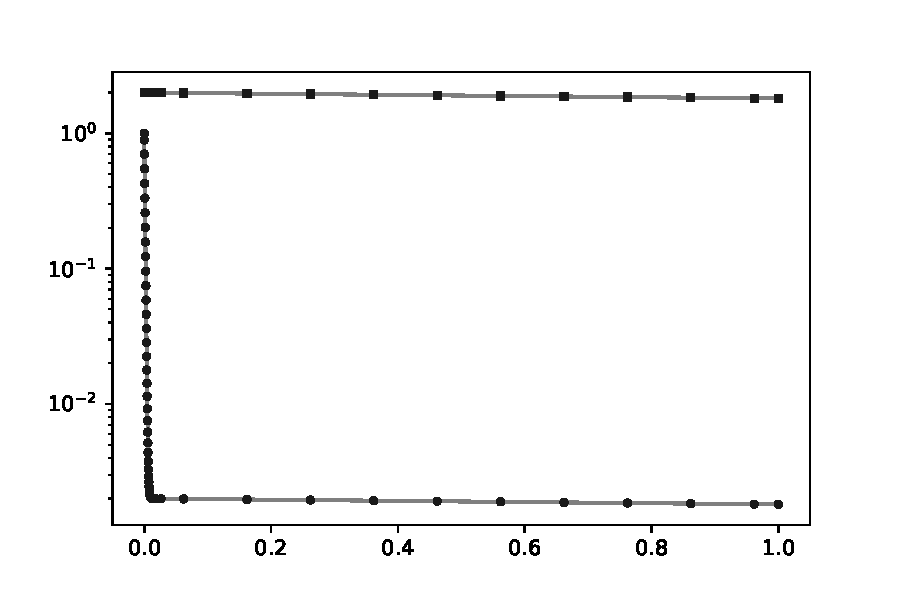
\includegraphics[width=\textwidth]{img/5/ode23s.pdf}
            \caption{{\tt ode23s} solution,  \( N=51 \), error = 0.00923}
            \label{rk23}
        \end{subfigure}
        \begin{subfigure}{.48\textwidth}\centering
            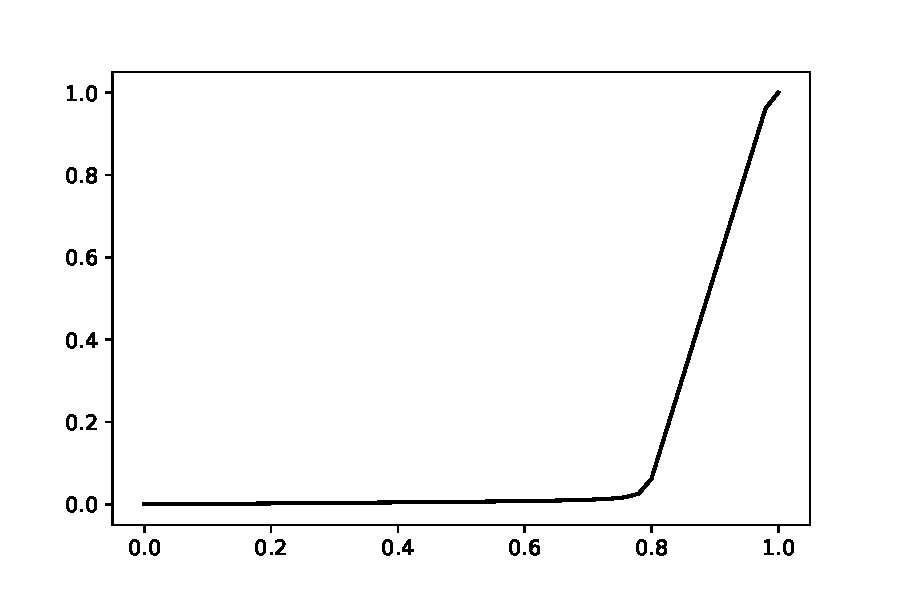
\includegraphics[width=\textwidth]{img/5/ode23s_t.pdf}
            \caption{linear time steps vs time steps from RK23}
            \label{rk23t}
        \end{subfigure}
    \caption{}
    \end{figure}


\end{enumerate}

\end{solution}
\end{document}
